%------------------------------------------------------------
% Description : Важные формулки, просто так
% Author      : Iliya Tikhonenko <iliya.t@mail.ru>
% Created at  : Sat Jun 17 14:33:58 MSK 2017
%------------------------------------------------------------
\documentclass[final,landscape,hardcopy]{notes}
\usepackage{tmath}
\usepackage{cussymb}
\usepackage{multicol}
\usepackage{bm}
\geometry{
  left=0.7cm,
  right=0.7cm,
  top=0.7cm,
  bottom=0.7cm
}
\graphicspath{{img/}}
\everymath{\displaystyle}
\usepackage{endnotes}
\renewcommand{\footnote}{\endnote}
\setlist[enumerate,1]{leftmargin=0pt, labelwidth=*}
\setlist[itemize,1]{leftmargin=0cm, noitemsep, label=$\triangleright$}
\setlength{\columnsep}{2em}
\setlength{\columnseprule}{0.0pt}
\begin{document}
\begin{multicols*}{4} \raggedright
\begin{enumerate}
  \item 
    \begin{description}
      \item[$\v r$:] $\v r(t)$, $(x,y,z)(t)$, $\v r(s)$.
      \item[$\dot{\v r}$:] $\dot{\v r}(t)$, $(\dot x,\dot y,\dot z)(t)$, $\v\tau \dot s$.
      \item[$\ddot{\v r}$:] $\ddot{\v r}(t)$, $(\ddot x,\ddot y,\ddot z)(t)$,
        $\ddot s \v \tau + \dot s^2 k_1 \v n$
    \end{description}
  \item В криволинейных координатах
    \begin{itemize}
      \item $\v e^k \cdot \v e_j = \delta_{kj} $, $\v a \cdot \v b = \sum_i a^i b_i $
      \item $\xi_k = \v r\cdot \v e_k = \sum_j \xi^j g_{jk}$,
        $\xi^k = \v r\cdot \v e^k = \sum_j \xi_j g^{jk}$
      \item $\v e^k = \sum_j g^{jk} e_j$, $\v e^k = \sum_j g^{jk} e^j$
      \item $\sum_i g^{i\ell}\, g_{ik} = \delta_{\ell k}$
    \end{itemize}
  \item Скорость и ускорение 
    \begin{itemize}[$\triangleright$]
      \item $\v v = \sum_k \dot q^k \v {e_k}$
      \item $\v w = \sum_k \ddot q^k \v e_k + \sum_{k,i} \dot q^k \dot q^i \, \pder{\v e_k}{q^i}$
      \item ${w^j} = \ddot q^j + \sum_{k,i} \dot q^k \dot q^i \, \Gamma_{ki}^j$
      \item $ \Gamma_{j,\,ki} = \pder{\v e_k }{q^i}\cdot \v e_j$~--- I рода
      \item $ \Gamma_{ki}^j \;\,\,= \pder{\v e_k }{q^i}\cdot \v e^j$~--- II рода
      \item $w_\ell = 
        \fder{}{t} \left(\pder{}{\dot q^\ell}\left(\frac{\dot{\v r}^2}{2}\right)\right) 
        - \fder{}{q^\ell} \left(\frac{\dot{\v r}^2}{2}\right)$
    \end{itemize}
  \item Про углы Эйлера \\
    \noindent

    \begin{itemize}[$\triangleright$]
      \item $\v \omega = \dot\psi\,\v i_3'  + \dot\theta\,\v i_1''  + \dot\varphi\,\v i_3  $
      \item $\v R (t) = \v R_0  (t) + \v r(t)$
      \item $\v v = \v {v_0} + \v \omega \times \v r  + \v v_r $
      \item $\v w = \v w_0 + \dot{\v \omega} \times \v r 
        + \v \omega \times (\v \omega \times \v r) + 2 \v \omega \times \v v_r  + \v w_r $
    \end{itemize}
    
    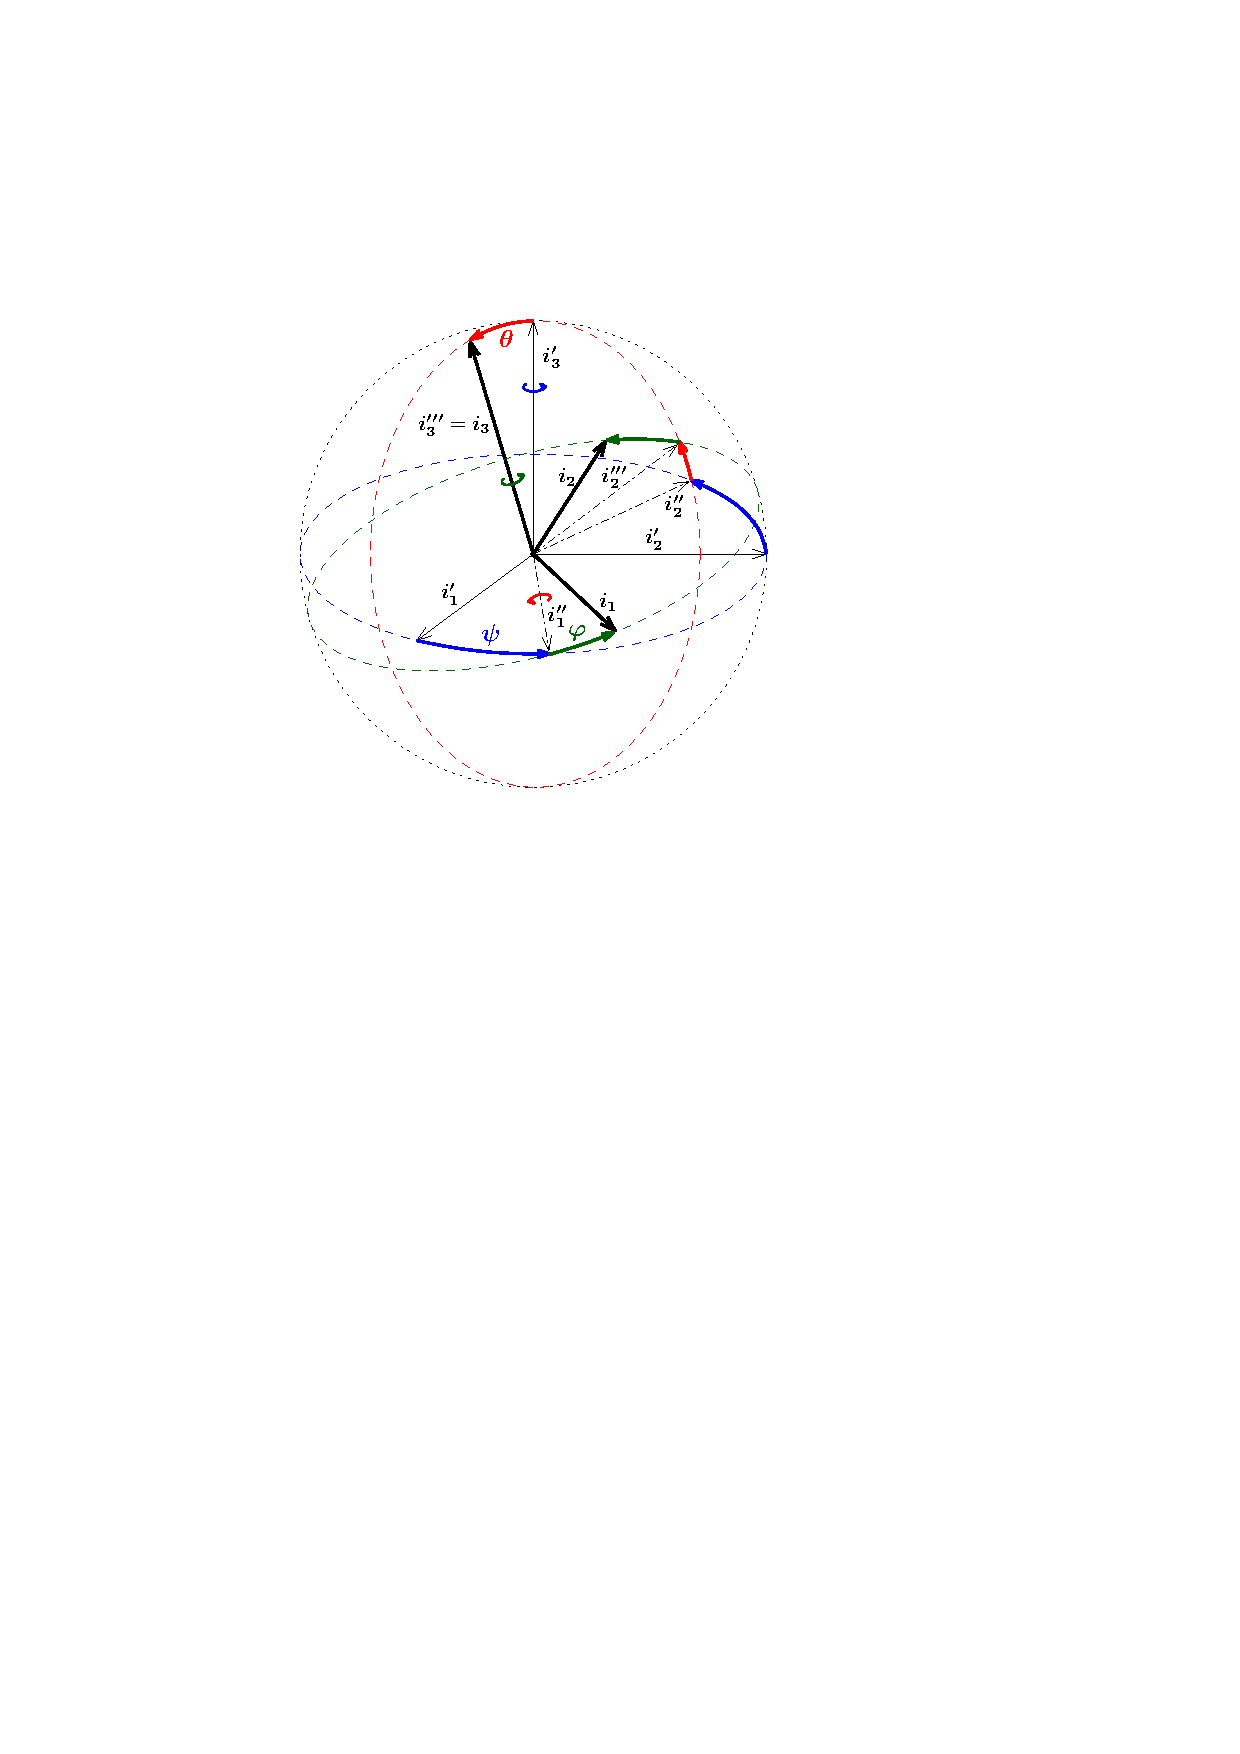
\includegraphics[width=1.0\linewidth]{euler_ang.pdf}
  
  \item Динамика точки и систем точек
    \begin{itemize}
      \item $\v r_k = \v r_k (t, \{c_\ell\})$, $k\in 1 \intrng N$, $\ell \in 1 \intrng 6N$
      \item $m_k \ddot{\v r_k} = \v F_k$, $m w_\ell= Q_\ell$
      \item $\fder{}{t} \left(\pder{T}{\dot q^\ell}\right) 
        - \fder{T}{q^\ell}  = Q_\ell$
      \item $\v r_c = \frac{\sum_k m_k \v r_k}{\sum_k m_k} $, $\sum_k m_k = M$
    \end{itemize}
  \item Закон сохранения импульса
    \begin{itemize}
      \item $\v p = \sum_k \v p_k$, $\v p_k = m_k \v v_k$
      \item $\v F = \sum_k \left( \v F_k^{(e)} + \v F_k^{(i)}\right)$
      \item $\fder{\v p}{t} = \sum_k \v F_k^{(e)}$. Все сиды взаимодействия вымерли.
    \end{itemize}
  \item  Момент импульса
    \begin{itemize}
      \item $\v \ell = \sum_k \v\ell_k $, $\v \ell_k = \v r_k \times \v p_k $
      \item $\v L = \sum_k \v r_k \times \v F_k^{(e)} + \sum_k \v r_k \times \v F_k^{(i)}  $
      \item $\v F_{kj}^{(i)} = \lambda (\v r_{kj}) \v r_{kj}$ $ \Rightarrow $ 
        $\fder{\v \ell}{t} = \sum_k \v L_k^{(e)}$.
    \end{itemize}
  \item Энергия
    \begin{itemize}
      \item $T = \sum_k T_k$, $T_k = \frac{m_k (\v v_k \cdot \v v_k)}{2}$
      \item $\delta A_k = \v F_k \cdot \del \v r_k$, 
        $A = \int_\Gamma \delta A$, а вообще-т интеграл от формы.
      \item $\del T = \delta A_k^{(e)} + \delta A_k^{(i)} $
      \item $\del E = \del \left(T + \Pi^{(e)} + \Pi^{(i)}\right) = \delta A_{\text{не\,пот}}$
    \end{itemize}
  \item В поле центральной силы$\neg$
    \begin{itemize}[$\triangleright$]
      \item $u = 1/\rho$.
      \item  Формулы Бине \\
        $\left\{\begin{aligned}
          v^2 &= c^2 \left(\left(\fder{u}{\varphi}\right)^2 + u^2 \right) \\
          w_\rho &= -c^2 u^2 \left(\fder[2]{u}{\varphi} + u \right)
      \end{aligned}\right.$
    \item Невыразимая жжесть
    \end{itemize}
  \item \quest\flame Движение твёрдого тела $\neg$
    \begin{itemize}
    \raggedright
      \item $\omega =0$~--- поступательное
      \item $\v {v_0}, \v {w_0} =0, \omega = \dot \varphi \v i_3 $~--- вращение вокруг неподвижной оси
      \item $\v {v_0} \coori \v \omega $~--- винт
      \item Как попало вокруг неподвижной точки\footnote{У нас тут вроде косяк, 
        а дальше снова как здесь \sour}$\neg$ 
        $\begin{aligned}
          \v \omega 
          &= \v i_1  (\dot \psi \sin \theta \sin \varphi + \dot \theta  \cos \varphi ) + \\
          &+ \v i_2  (\dot \psi \sin \theta \cos \varphi - \dot \theta \sin \varphi ) + \\
          &+ \v i_3  (\dot \psi \cos \varphi + \dot \varphi )
      \end{aligned}$
    \end{itemize}
  \item Скорость и ускорение точек твердого тела
    \begin{itemize}
      \item $\v v = \v {v_0} + \v {\omega \times r}$
      \item $\v w = \v {w_0} + \dot{\v\omega} \times \v r + \v\omega \times (\v\omega \times \v r)$
    \end{itemize}
  \item Сложение движений ТТ
    \begin{itemize}
      \item $\v {v_{r_n}} 
        = \sum_{k=0}^{n-1} \left( \v v_k  + \v \omega_k  \times \ov{->}{O_kO}\right) 
        + \sum_{k=0}^{n-1} \v \omega_k  \times \v r_0 $, $O_0 = O$.
      \item $\v V  = \sum_{k=0}^{n-1} \left( \v v_k  + \v \omega_k  \times \ov{->}{O_kO}\right) $
      \item $\v \Omega   = \sum_{k=0}^{n-1} \v \omega_k  \quad\Rightarrow \v {v_{r_n}} 
        = \v V + \v\Omega \times \v r_0 $
    \end{itemize}
  \item Кинематический винт
    \begin{itemize}
      \item $\v \omega \times \v v_0 + \v \omega \times (\v \omega \times \v r)= 0$
    \end{itemize}
  \item Плоское  движение
    \begin{itemize}
      \item $0 = \v v_0 + \v \omega \times \v r_c $ 
      \item $\v r_* = \left(-\frac{v_{0y}}{\omega}, + \frac{v_{0x}}{\omega}\right)$~---подвижная 
        центроида
      \item $\v r_*' = \v r_* + \v r_0 $~--- неподвижная центроида
      \item $\omega = \frac{|\v v_B - \v v_A|}{|\v r_B - \v r_A|}$
      \item $\omega = \frac{|\v v_a \times \v r_{A*}|}{r_{A*}^2} $ и то же с $B$.
      \item центр ускорений: \quest
    \end{itemize}
  \item Динамика вращения ТТ
    \footnote{Здесь по-хорошему надо меру на многобразии вводить}
    \begin{itemize}
      \item $M = {\dint_\tau  1 \, \del \mu(r) }$
      , $\v r_c = \frac{\dint_\tau \v r \, \del \mu(r)}{\dint_\tau  1 \, \del \mu(r) } $
      \item $\v {\ell} = \int_\tau (\v r \times (\v \omega \times \v r) \, \del \mu$,
        $\v \ell' = \int_\tau (\v R \times \v v) \, \del \mu$
      \item $
          \v \ell' = \v R_0 \times \v v_0 \, M + \v r_c \times \v v_0 \, M + \v R_0 
          \times (\v \omega \times \v r_c) M + \ell
        $
      \item $T  = \frac 1 2 \int_\tau (\v \omega \times \v r)^2 \, \del \mu$,
            $T' = \frac 1 2 \int_\tau {\v v}^2 \, \del \mu$
      \item $T' = T + \frac 1 2 M \v v_0^2 + M \v v_0 \cdot (\v \omega \times \v r_c)$
      \item $\ell_\omega = \omega J_\omega  $
      \item $\v \ell = \ov^ J \v \omega = \sum_{j,k} J_{jk} \omega_k \,\v i_j$, 
        $J_{ik} = \int_\tau (r^2 \delta_{jk} - x_j x_k) \, \del \mu $
      \item $T = \frac{J_\omega \omega ^2}{2} = \frac{\ov^ J \, \v \omega \cdot \v \omega}{2} $
      \item $L = \fder{\ell}{t}$
      \item Динамические уравнения Эйлера $\neg$ \\
        $
        \begin{aligned}
          L_a &= J_a \dot \omega _a + (J_c - J_b)\, \omega_c \omega_b \\ 
          L_b &= J_b \dot \omega _b + (J_a - J_c)\, \omega_a \omega_c \\ 
          L_c &= J_c \dot \omega _c + (J_b - J_a)\, \omega_b \omega_a 
        \end{aligned}
        $
      \item Кинематические уравнения Эйлера $\neg$ \\ 
        $
        \begin{aligned}
          \label{eq:kineuler}
          \omega_a &= (\dot \psi \sin \theta \sin \varphi + \dot \theta  \cos \varphi )  \\
          \omega_b &= (\dot \psi \sin \theta \cos \varphi - \dot \theta \sin \varphi )  \\
          \omega_c &= (\dot \psi \cos \varphi + \dot \varphi )
        \end{aligned}
        $
    \end{itemize}
  \item Вращение вокруг неподвижной оси$\neg$
    \begin{itemize}
      \item $m \fder{\v v_c}{t} = \v F + \v N_A + \v N_B$, $\v v_c = \v \omega \times \v r_c$, $ \Rightarrow $
        $
        \begin{aligned}
          m(-\ddot \varphi x_{c_2} + (\dot \varphi)^2 x_{c_1}) &=  F_1 +  N_{A_1} +  N_{B_1}\\
          m(\ddot \varphi x_{c_1} - (\dot \varphi)^2 x_{c_2}) &=  F_2 +  N_{A_2} +  N_{B_2}\\
          0 &=  F_3 +  N_{A_3} +  N_{B_3}
        \end{aligned}
        $
      \item $\fder{\v \ell}t = \v L + (\v r_A \times \v N _A)+ (\v r_A \times \v N _A) \Rightarrow $
        $
        \begin{aligned}
          J_{13} \ddot \varphi - J_{23}(\dot \varphi)^2  &=  L_1 - r_A N_{A_2} +  r_B N_{B_2}\\
          J_{23} \ddot \varphi + J_{13}(\dot \varphi)^2  &=  L_2 + r_A N_{A_1} -  r_B N_{B_1}\\
          J_{33} \ddot \varphi &= L_3
        \end{aligned}
        $
    \end{itemize}
  \item $L = 0$
    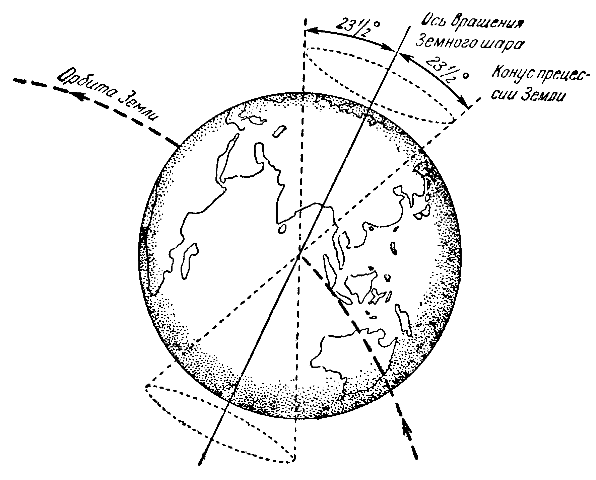
\includegraphics[width=\linewidth]{earth}   
  \item Сила всего одна и приложена к центру масс\\
    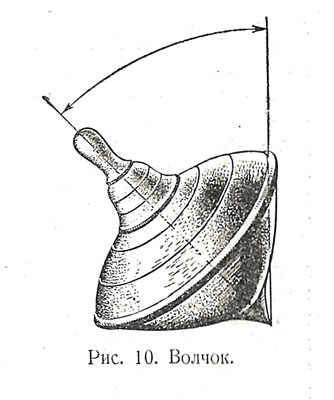
\includegraphics[width=0.7\linewidth]{lagrset2}
    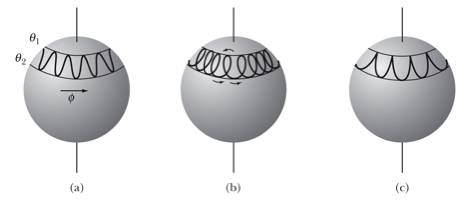
\includegraphics[width=\linewidth]{largtraj2}
  \item Связи
    \begin{itemize}
      \item $\varphi(t,\v r, \v v) \geqslant 0$ (или $=0$)
      \item $\varphi(t,\v r, \v v) = 0 \Leftrightarrow f(t, \v r) = 0$~---~голономные 
      \item $\v R_i = \Lambda_i \nabla' \varphi_i + \v T_i$, \footnote{Здесь вообще градиенты, но жирная 
        набла выглядит некрасиво: $\v \nabla\varphi $}
        $\Lambda_i = -\frac{m\pder{\varphi_i}t + m\nabla \varphi_i \v v + \nabla' \varphi_i \v F }
        {|\nabla' \varphi_i|^2}$
    \end{itemize}
  \item По поверхности
    \begin{itemize}
      \item $m \v w= \v F + \Lambda \nabla f + \v T$
      \item $\v T = -k N \v\tau$
      \item $\v F = 0$, $v^2 = v_0^2 e^{-\alpha(s)}$
    \end{itemize}
  \item По кривой 
    \begin{itemize}
      \item $m \v w= \v F + \Lambda_1 \nabla f_1 +\Lambda_2 \nabla f_2 + \v T$
      \item $\v T = -k N \v\tau$
      \item катится мир к упадку
    \end{itemize}
  \item Принцип Даламбера-Лагранжа: \\
    Суммарная работа сил инерции и активных сил по виртуальным перемещениям равна нулю:
    $
    (M \ddot{\v y} - \v Y ) \cdot \delta \v y = 0
    $
  \item При варьировании с фиксированными концами $\Bigg(\delta t_1 = \delta t_0 = 0$, 
      $
      \begin{aligned}
        \delta q^\ell |_{t_1} = 0 \\ \delta q^\ell |_{t_2} = 0 
      \end{aligned}
    \Bigg)
    $
    $\delta S = 0 \Leftrightarrow \fder{}{t}\, \left(\pder{L}{\dot q^l}\right) - \pder{L}{q^l} = 0$
  \item Интегральный принцип Лагранжа:
    \begin{itemize}
      \item $\delta W = \delta \int_{t_0}^{t_1} 2 T$, 
        $T = \tfrac{M}{2} \sum_{j,k} g_{ij} \dot q^j \dot q^k$
      \item $\delta q_0^\ell = \delta q_1^\ell = 0 \Rightarrow \Delta q|_{t_1} = \Delta q |_{t_0}$,
        $\Delta q^\ell = \delta q^\ell + \dot q^\ell \delta t$ (полная вариация)
      \item Лишь при этом условии работает принцип выше
    \end{itemize}
  \item $\pder{S}{t} + H\left(q^\ell ,\pder{S}{q^\ell}, t\right) = 0$
  \item $
    \left\{
      \begin{aligned}
        \label{eq:hamilt}
        \dot q^k &= \pder{H}{p_k} \\
        \dot p_k &= - \pder{H}{q^k} + Q_k
      \end{aligned}
    \right.
    $
  \item Теорема Якоби \\
    \hspace{-1.2em}$ 
    \left\{
      \begin{aligned}
        \label{eq:jacobth}
        &\pder{S}{t} + H\left(q^\ell ,\pder{S}{q^\ell}, t\right)= 0, \\
        &\det\left(\pdder{S}{q^l}{a^p}\right) \neq 0\quad\Rightarrow~\\ 
        &p_\ell = \pder{S}{q^\ell}, \; b_k = \pder{S}{a^k}\\
        &a_k, b_k \text{~--- const}
      \end{aligned}
    \right.~
    \left\{
      \begin{aligned}
        \label{eq:hamilt}
        \dot q^k &= \pder{H}{p_k} \\
        \dot p_k &= - \pder{H}{q^k}
      \end{aligned}
    \right.
    $
  \item Инварианты
    \begin{itemize}
      \item Ф.~объём:
        $\int_M \rho \, \del \Omega $, $\del \Omega =``\prod_i" \del q^i\,\del p_i $
      \item Пуанкаре: $\oint_C p_k \, \del q^k$
      \item Пуанкаре-Картане: $\oint_C p_k \, \del q^k-H\del t$
    \end{itemize}
    Здесь \\
    $M$~--- сечение фазовой трубки,\\ 
    $C$~--- охватывающий её контур.
  \item Канонические преобразования\par
    Когда нету зависимости от времени
    \begin{itemize}
      \item $p_k = p_k(\ov~p, \ov~q)$, $q^k = q^k(\ov~p, \ov~q)$, 
        $\ov~H(t, \ov~p, \ov~q)=  H\bigl(t, p(\ov~p, \ov~q), q(\ov~p, \ov~q)\bigr)$
    \end{itemize}

    Когда есть порождающая функция $V$.
    \begin{enumerate}[1*,start=0]
      \item $\ov~L = L + \fder{V}{t}$
      \item $V_1(t,q,\ov~q)=V$ 
      \item $V_2(t,p,\ov~q)=V+\sum_k p_k q^k$ 
      \item $V_3(t,\ov~p,q)=V-\sum_k \ov~p_k \ov~q^k$ 
      \item $V_4(t,p,\ov~p)=V + \sum_k p_k q^k- \sum_k \ov~p_k \ov~q^k$ 
    \end{enumerate}
    
    При этом
    \begin{enumerate}[$ \langle 1 \rangle $, leftmargin=2ex]
      \item $\ov~p_k = +\pder{V_1}{\ov~q^k}$, $p_k = +\pder{V_1}{q^k}$, $\ov~H = H - \pder{V_1}{t}$
      \item $\ov~p_k = +\pder{V_2}{\ov~q^k}$, $q^k = -\pder{V_2}{p_k}$, $\ov~H = H - \pder{V_2}{t}$
      \item $\ov~q^k = -\pder{V_3}{\ov~p_k}$, $p_k = -\pder{V_3}{q^k}$, $\ov~H = H - \pder{V_3}{t}$
      \item $\ov~q^k = -\pder{V_4}{\ov~p_k}$, $q^k = +\pder{V_4}{p_k}$, $\ov~H = H - \pder{V_4}{t}$
    \end{enumerate}
    Выглядит не очень, но бывают вещи и похуже
\end{enumerate}

\theendnotes

\end{multicols*}
\end{document}
% vim:tw=100 cc=100
